\chapter{Álgebra \texorpdfstring{$\ZZ$}{ℤ}-lineal}

Dedicamos el capítulo anterior al álgebra conmutativa, y ahora nos ocuparemos
de\dots{} álgebra lineal. Recordemos que para una extensión finita de campos
$L/K$, la norma y traza de un elemento $\alpha \in L$ se definen como el
determinante y traza de la aplicación $K$-lineal $x \mapsto \alpha x$.
Ahora vamos a explorar estas construcciones para extensiones de anillos.

%%%%%%%%%%%%%%%%%%%%%%%%%%%%%%%%%%%%%%%%%%%%%%%%%%%%%%%%%%%%%%%%%%%%%%%%%%%%%%%%

\pdfbookmark{Clase 9 (07/09/20)}{clase-9}
\section{Norma y traza}
\marginpar{\small Clase 9 \\ 07/09/20}

\begin{definicion}
  Sea $A \subset B$ una extensión de anillos tal que $B$ es un $A$-módulo libre
  de rango $n$ sobre $A$. Para $\beta \in B$ consideremos la aplicación
  $A$-lineal de multiplicación por $\beta$:
  $$\mu_\beta\colon B \to B, \quad x \mapsto \beta x.$$
  La \textbf{norma} y \textbf{traza} de $\beta$ se definen como el determinante
  y traza de $\mu_\beta$ respectivamente:
  $$N_{B/A} (\beta) = \det \mu_\beta, \quad T_{B/A} (\beta) = \tr \mu_\beta.$$
  Esto nos da aplicaciones
  $$N_{B/A}, T_{B/A}\colon B\to A.$$
\end{definicion}

Específicamente, si $e_1, \ldots, e_n$ es una base de $B$ sobre $A$ y
$\beta \, e_i = \sum_j m_{ij} e_j$, entonces
$$N (\beta) = \det (m_{ij})_{i,j}, \quad T (\beta) = \sum_i m_{ii}.$$

El argumento habitual demuestra que esto no depende de la elección de base:
si $T$ es una matriz de cambio de base, entonces es invertible, y luego
\begin{gather*}
  \det (T M T^{-1}) = \det (T) \, \det (M) \, \det (T)^{-1} = \det (M),\\
  \tr (T M T^{-1}) = \tr (T^{-1} T M) = \tr (M).
\end{gather*}

Vamos a denotar el polinomio característico correspondiente por
$$f^\beta_{B/A} = \det (x I_n - M).$$
Este es un polinomio mónico de grado $n$:
$$f^\beta_{B/A} = x^n + a_{n-1} x^{n-1} + \cdots + a_1 x + a_0 \in A [x].$$
El argumento habitual demuestra que
\begin{equation}
  \label{eqn:norma-y-traza-coeficientes-de-polinomio-caracteristico}
  a_0 = (-1)^n \, N_{B/A} (\beta), \quad a_{n-1} = -T_{B/A} (\beta).
\end{equation}

La norma es multiplicativa:
$$N (\beta \beta') = N (\beta)\,N(\beta'),$$
mientras que la traza es $A$-lineal:
\[ T (a \beta) = a \, T (\beta), \quad
   T (\beta+\beta') = T (\beta) + T (\beta'). \]
Para $a \in A$ se tiene
$$N (a) = a^n, \quad T (a) = na.$$

\begin{proposicion}
  Para un campo de números $K/\QQ$ tenemos $n = [K : \QQ]$ encajes
  $$\sigma_1,\ldots,\sigma_n\colon K \hookrightarrow \CC,$$
  y la norma y traza vienen dadas por
  \[ N_{K/\QQ} (\alpha) = \sigma_1 (\alpha) \cdots \sigma_n (\alpha), \quad
     T_{K/\QQ} (\alpha) = \sigma_1 (\alpha) + \cdots + \sigma_n (\alpha). \]
  Aquí $\sigma_i (\alpha)$ son las raíces del polinomio característico
  de $\alpha$ respecto a la extensión $K/\QQ$.

  \begin{proof}
    Primero, si $K = \QQ (\alpha)$, entonces un encaje
    $\sigma\colon K \hookrightarrow \CC$ está definido por la imagen de
    $\alpha$ y tiene que enviarlo a una raíz compleja del polinomio
    mínimo $f_\QQ^\alpha$. De esta manera surgen los
    $[K (\alpha) : \QQ]$ encajes. Tenemos
    \[ f_\QQ^\alpha =
       \prod_{\sigma\colon K\hookrightarrow \CC} (x - \sigma (\alpha)). \]

    En general, tenemos $\QQ \subset \QQ (\alpha) \subset K$, y cada
    encaje $\sigma\colon \QQ (\alpha) \hookrightarrow \CC$ admite
    $[K : \QQ (\alpha)]$ extensiones a un encaje $K \hookrightarrow \CC$.
    Ahora
    \[ f^\alpha_{K/\QQ} = (f^\alpha_\QQ)^{[K : \QQ (\alpha)]} =
       \prod_{\sigma\colon K\hookrightarrow \CC} (x - \sigma (\alpha)), \]
    donde $f^\alpha_{K/\QQ}$ es el polinomio característico, mientras que
    $f^\alpha_\QQ$ es el polinomio mínimo.
    En fin, recordemos cómo la norma y traza están relacionadas con los
    coeficientes del polinomio característico (las fórmulas
    \eqref{eqn:norma-y-traza-coeficientes-de-polinomio-caracteristico}).
  \end{proof}
\end{proposicion}

\begin{comentario}
  Dado que $K/\QQ$ es una extensión algebraica, en realidad todo encaje
  $\sigma\colon K \hookrightarrow \CC$ tiene su imagen en $\overline{\QQ}$,
  la cerradura algebraica de $\QQ$, así que los números complejos no son
  tan relevantes.

  Si $K/\QQ$ es una extensión de Galois, entonces los encajes
  $K \hookrightarrow \CC$ corresponden a los elementos de $\Gal (K/\QQ)$.
  En general, puede haber más encajes que automorfismos de Galois.

  Para revisar más detalles sobre la norma y traza de una extensión finita de
  campos, el lector puede revisar, por ejemplo,
  \cite[\S II.8]{Morandi-GTM167} o \cite[\S VI.5]{Lang-Algebra}.
\end{comentario}

\begin{proposicion}
  Si $\alpha \in \O_K$, entonces
  $N_{K/\QQ} (\alpha), T_{K/\QQ} (\alpha) \in \ZZ$.

  \begin{proof}
    Si $\alpha_1, \ldots, \alpha_n$ son las raíces del polinomio característico
    de $\alpha$ sobre $\QQ$, entonces estas son también enteros algebraicos,
    y por lo tanto $N (\alpha) = \alpha_1\cdots\alpha_n$ y
    $T (\alpha) = \alpha_1 + \cdots + \alpha_n$ son enteros algebraicos.
    Al mismo tiempo son números racionales, así que
    $N (\alpha), T (\alpha) \in \ZZ$.
  \end{proof}
\end{proposicion}

\begin{proposicion}
  Se tiene
  $$\O_K^\times = \{ \alpha \in \O_K \mid N (\alpha) = \pm 1 \}.$$

  \begin{proof}
    Si $\alpha \in \O_K$ tiene inverso $\alpha^{-1} \in \O_K$, entonces
    $$N (\alpha)\, N (\alpha^{-1}) = N (\alpha\alpha^{-1}) = 1.$$
    Pero $N (\alpha^{\pm 1}) \in \ZZ$, así que $N (\alpha) = \pm 1$.
    Viceversa, si $\alpha \in \O_K$ y $N (\alpha) = \pm 1$, sean
    $\alpha_1 = \alpha$, $\alpha_2$, $\ldots$, $\alpha_n$ las raíces
    del polinomio característico de $\alpha$. Tenemos
    $$\alpha \alpha_2 \cdots \alpha_n = \pm 1,$$
    y luego
    $$\alpha^{-1} = \pm (\alpha_2 \cdots \alpha_n),$$
    donde $\alpha_i$ son enteros algebraicos, así que el producto a la derecha
    está en $\O_K$\footnote{No estamos diciendo que cada $\alpha_i$ está en
      $K$; esto sucede cuando $K/\QQ$ es una extensión de Galois.}.
  \end{proof}
\end{proposicion}

\begin{ejemplo}
  Consideremos el campo cuadrático $K = \QQ (\sqrt{d})$, donde $d$ es libre de
  cuadrados. La multiplicación por $a + b\sqrt{d}$ en la base $1, \sqrt{d}$ se
  representa por la matriz
  \[ \begin{pmatrix}
    a & db \\
    b & a
  \end{pmatrix}. \]
  Entonces,
  \[ N (a + b\sqrt{d}) = a^2 - db^2, \quad
     T (a + b\sqrt{d}) = 2a. \]
  También calculamos
  \[ (a + b\sqrt{d})\,(a - b\sqrt{d}) = a^2 - db^2, \quad
     (a + b\sqrt{d}) + (a - b\sqrt{d}) = 2a. \qedhere \]
\end{ejemplo}

%%%%%%%%%%%%%%%%%%%%%%%%%%%%%%%%%%%%%%%%%%%%%%%%%%%%%%%%%%%%%%%%%%%%%%%%%%%%%%%%

\section{Recordatorio de álgebra lineal}

Sea $V$ un espacio vectorial de dimensión finita sobre un campo $k$.
Consideremos una forma bilineal simétrica
$$\langle\cdot,\cdot\rangle\colon V\times V\to k.$$

Sea $e_1,\ldots,e_n$ una base de $V$. El \textbf{discriminante} de
$\langle\cdot,\cdot\rangle$ respecto a esta base se define como
$$\Delta (e_1,\ldots,e_n) = \det (\langle e_i,e_j\rangle)_{i,j}.$$

El discriminante depende de la base. En general, si $f_1,\ldots,f_n$ son algunos
elementos de $V$ y $f_i = \sum_j a_{ij} e_j$, entonces calculamos que
\[ \langle f_k,f_\ell\rangle =
   \langle \sum_i a_{ki} e_i, \sum_j a_{\ell j} e_j \rangle =
   \sum_{i,j} a_{ki} \, \langle e_i, e_j\rangle \, a_{\ell j}. \]
En términos de matrices,
\[ (\langle f_i,f_j\rangle)_{i,j} =
   (a_{ij}) \cdot (\langle e_i, e_j\rangle)_{i,j} \cdot (a_{ij})^t. \]
Luego,
\[ \det (\langle f_i,f_j\rangle)_{i,j} =
   \det (a_{ij})_{i,j}^2 \cdot \det (\langle e_i, e_j\rangle)_{i,j}. \]
También recordemos que $f_1,\ldots,f_n$ es otra base de $V$ si y solamente si
$\det (a_{ij})_{i,j} \ne 0$.

Se dice que la forma $\langle\cdot,\cdot\rangle$ es \textbf{no degenerada}
si se cumple una de las siguientes condiciones equivalentes:
\begin{enumerate}
\item[1)] el discriminante de $\langle\cdot,\cdot\rangle$ respecto a alguna
  base de $V$ no es nulo;
\item[2)] $\langle\cdot,\cdot\rangle$ induce un isomorfismo entre $V$ y el
  espacio dual $V^\vee = \Hom_k (V,k)$ mediante
  \[ \phi\colon V \xrightarrow{\cong} V^\vee, \quad
     v \mapsto (x \mapsto \langle v,x\rangle). \]
\end{enumerate}

Ahora supongamos que se cumplen estas condiciones. Recordemos que el espacio
dual $V^\vee$ tiene base $e_1^*, \ldots, e_n^*$ definida por
\[ e_i^* (e_j) = \delta_{ij} = \begin{cases}
  1, & \text{si } i = j,\\
  0, & \text{si } i \ne j.
\end{cases} \]
Usando el isomorfismo $\phi\colon V \cong V^\vee$ de arriba, podemos tomar
los vectores $e_i' = \phi^{-1} (e_i^*)$, y luego $e_1', \ldots, e_n'$ cumplen
$$\langle e_i', e_j\rangle = \delta_{ij}.$$
Podemos decir que $e_1', \ldots, e_n'$ es la base \textbf{dual} a
$e_1, \ldots, e_n$ respecto a la forma bilineal.

%%%%%%%%%%%%%%%%%%%%%%%%%%%%%%%%%%%%%%%%%%%%%%%%%%%%%%%%%%%%%%%%%%%%%%%%%%%%%%%%

\section{Apareamiento de traza y el discriminante}

\begin{definicion}
  Para una extensión de anillos $A \subset B$ tal que $B$ es un $A$-módulo libre
  de rango $n$, el \textbf{apareamiento de traza}\footnote{En la primera
    versión de estos apuntes decía ``emparejamiento'' y luego me di cuenta de
    que en México es más común el término ``apareamiento''.}  es la forma
  $A$-bilineal simétrica
  \[ \langle\cdot,\cdot\rangle\colon B\times B\to A, \quad
     (x,y) \mapsto T_{B/A} (xy). \]
  Para una base $e_1,\ldots,e_n$ de $B$ sobre $A$, el \textbf{discriminante}
  viene dado por
  \[ \Delta (e_1,\ldots,e_n) =
     \det (\langle e_i,e_j\rangle)_{i,j}. \]
\end{definicion}

Si $f_1, \ldots, f_n$ son otros elementos que se expresan en términos de los
$e_i$ mediante $f_i = \sum_j a_{ij} e_j$, entonces los mismos cálculos que vimos
arriba nos dan la relación
\[ \Delta (f_1,\ldots,f_n) =
   \det (a_{ij})_{i,j}^2 \cdot \Delta (e_1,\ldots,e_n). \]
Ahora $f_1,\ldots,f_n$ es una base si y solamente si $(a_{ij})_{i,j}$ es una
matriz invertible, lo que equivale a $\det (a_{ij})_{i,j} \in A^\times$.
Entonces, si no queremos fijar una base particular, el discriminante está bien
definido solamente salvo un factor de $(A^\times)^2$, como un elemento de
$A^\times/(A^\times)^2$.

Sin embargo, en el caso particular cuando $A = \ZZ$, tenemos $(A^\times)^2 = 1$,
así que el discriminante es un número entero bien definido. Vale la pena
recordar esto como una definición. Como siempre nos interesan anillos de
números $R \subset K$.

\begin{definicion}
  Sea $R$ un anillo de números que es finitamente generado (y luego libre) como
  $\ZZ$-módulo. Entonces, \textbf{el~discriminante} de $R$ viene dado por
  $$\Delta (R) = \det (\langle \alpha_i, \alpha_j\rangle)_{i,j},$$
  donde $\alpha_1,\ldots,\alpha_n$ es alguna base de $R$ sobre $\ZZ$.
  (Como acabamos de notar, el resultado no depende de la base.)
\end{definicion}

\begin{lema}
  \label{lema:indice-de-Z-submodulo-como-determinante}
  Sea $R$ un $\ZZ$-módulo libre de rango $n$ con una base
  $\alpha_1,\ldots,\alpha_n$. Para $\beta_1,\ldots,\beta_n \in R$
  consideremos el $\ZZ$-submódulo generado por $\beta_1,\ldots,\beta_n$:
  $$M = \ZZ \langle\beta_1,\ldots,\beta_n\rangle.$$
  Tenemos $\beta_i = \sum_j a_{ij} \alpha_j$ para $a_{ij} \in \ZZ$.
  Entonces,
  \[ [R : M] = \begin{cases}
    \infty, & \text{si }\det (a_{ij})_{i,j} = 0, \\
    |\det (a_{ij})_{i,j}|, & \text{si }\det (a_{ij})_{i,j} \ne 0.
    \end{cases} \]

  \begin{proof}
    Podemos identificar $R$ con $\ZZ^n$ y el submódulo $M \subset R$
    con la imagen de una aplicación $\ZZ$-lineal $A\colon\ZZ^n \to \ZZ^n$
    (multiplicación por la matriz $A$).

    Primero, si $\det A = 0$, esto significa que hay una dependencia
    $\ZZ$-lineal entre los vectores de $M$, así que $\rk M < n$,
    y el índice de $M$ es infinito.

    Podemos poner $A$ en la \textbf{forma normal de Smith} (véase
    por ejemplo \cite[Chapter 2]{Cohen-GTM138})
    \[ B = \begin{pmatrix}
      b_1 \\
      & \ddots \\
      & & b_n
      \end{pmatrix} = U A V, \]
    donde $B$ es una matriz diagonal y $U, V \in \GL_n (\ZZ)$.
    Las aplicaciones $\ZZ$-lineales $U, V\colon \ZZ^n\to \ZZ^n$ son
    isomorfismos, así que $[\ZZ^n : A (\ZZ^n)] = [\ZZ^n : B (\ZZ^n)]$.
    Tenemos
    $$\det B = \det (U A V) = \pm\det (A),$$
    y luego
    \[ [\ZZ^n : B (\ZZ^n)] = \# (\ZZ/b_1\ZZ \times \cdots \times \ZZ/b_n\ZZ)
       = |\det B|. \qedhere \]
  \end{proof}
\end{lema}

\begin{ejemplo}
  Consideremos el subgrupo de $R = \ZZ^2$ generado por los vectores
  $\beta_1 = (2,3)$ y $\beta_2 = (-2,1)$. Estos corresponden a la matriz
  \[ A = \begin{pmatrix}
    2 & -2 \\
    3 & 1
  \end{pmatrix}. \]
  La forma normal de Smith en este caso
  será
  \[ \begin{pmatrix}
    1 & -6 \\
    0 & 1
  \end{pmatrix} \, \begin{pmatrix}
    2 & -2 \\
    3 & 1
  \end{pmatrix} \, \begin{pmatrix}
    1 & 1 \\
    -3 & -2
  \end{pmatrix} = \begin{pmatrix}
    8 & 0 \\
    0 & 1
  \end{pmatrix}. \]
  Entonces, el cociente de $\ZZ^2$ por $A (\ZZ^2)$ tiene $8$ elementos.
  Aquí están dibujados los vectores $\beta_1$ y $\beta_2$ y ocho representantes
  del cociente $\ZZ^2 / A (\ZZ^2)$.

  \begin{center}
    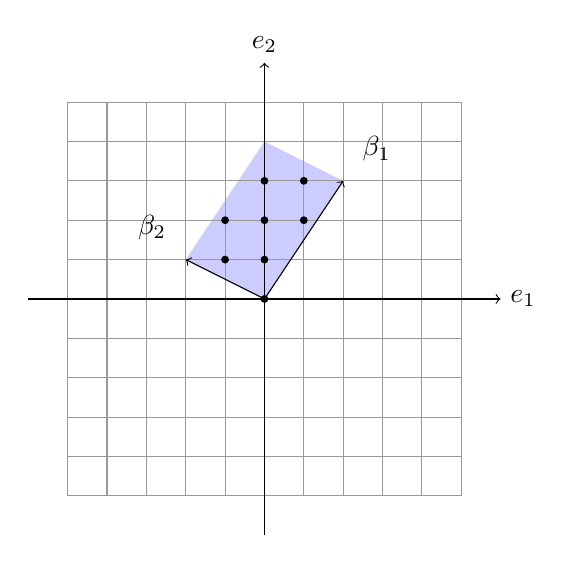
\begin{tikzpicture}[x=0.5cm,y=0.5cm]
        \fill[blue!20] (0,0) -- (2,3) -- (0,4) -- (-2,1) -- cycle;

        \foreach \i in {-5, ..., 5}
        \draw[black!40] (-5,\i) -- (5,\i);
        \foreach \i in {-5, ..., 5}
        \draw[black!40] (\i,-5) -- (\i,5);

        \draw[->] (-6,0) -- (6,0) node[right] {$e_1$};
        \draw[->] (0,-6) -- (0,6) node[above] {$e_2$};

        \draw[->] (0,0) -- (2,3) node [label={above right:$\beta_1$}] {};
        \draw[->] (0,0) -- (-2,1) node [label={above left:$\beta_2$}] {};

        \draw (-1,1) node[circle,fill,inner sep=1pt] {};
        \draw (-1,2) node[circle,fill,inner sep=1pt] {};
        \draw (0,0) node[circle,fill,inner sep=1pt] {};
        \draw (0,1) node[circle,fill,inner sep=1pt] {};
        \draw (0,2) node[circle,fill,inner sep=1pt] {};
        \draw (0,3) node[circle,fill,inner sep=1pt] {};
        \draw (1,2) node[circle,fill,inner sep=1pt] {};
        \draw (1,3) node[circle,fill,inner sep=1pt] {};
    \end{tikzpicture}
  \end{center}
\end{ejemplo}

Esto nos lleva al siguiente resultado.

\begin{proposicion}
  \label{prop:discriminantes-e-indice}
  Sea $R$ un anillo de números que es un $\ZZ$-módulo libre de rango $n$
  y $M \subseteq R$ un submódulo de rango $n$ generado por algunos elementos
  $\beta_1,\ldots,\beta_n$. Luego,
  $$\Delta (M) = [R : M]^2 \cdot \Delta (R).$$

  \begin{proof}
    $\Delta (M) = \Delta (\beta_1,\ldots,\beta_n) = \det (a_{ij})_{i,j}^2 \cdot \Delta (R)$,
    donde $|\det (a_{ij})| = [R : M]$.
  \end{proof}
\end{proposicion}

%%%%%%%%%%%%%%%%%%%%%%%%%%%%%%%%%%%%%%%%%%%%%%%%%%%%%%%%%%%%%%%%%%%%%%%%%%%%%%%%

\section{Generación finita del anillo de enteros}

Nuestro próximo objetivo es probar que para un campo de números
el apareamiento de traza no es degenerado y sacar algunas consecuencias
importantes de este resultado.
Primero necesitamos un lema bien conocido de la teoría de campos.

\begin{lema}[Dedekind; independencia lineal de caracteres]
  Dado un grupo abeliano $G$ y un campo $F$, consideremos diferentes caracteres
  multiplicativos $\chi_1,\ldots,\chi_n\colon G\to F^\times$. Estos son
  necesariamente linealmente independientes sobre $F$: si para algunos
  $c_1,\ldots,c_n \in F$ se cumple
  $$c_1 \chi_1 (g) + \cdots + \chi_n (g) = 0 \quad\text{para todo }g\in G,$$
  entonces $c_1 = \cdots = c_n = 0$.

  \begin{proof}
    Inducción sobre $n$, el caso base siendo $n = 1$. Supongamos que
    el resultado es válido para $n-1$ caracteres.
    Consideremos una dependencia lineal
    \[ \tag{*} c_1 \chi_1 (g) + \cdots + c_{n-1} \chi_{n-1} (g) + c_n \chi_n (g)
       = 0 \quad\text{para todo }g\in G. \]
    Dado que los caracteres son diferentes, existe $g_0 \in G$ tal que $\chi_1
    (g_0) \ne \chi_n (g_0)$. Sustituyendo $g_0 g$ en lugar de $g$, se obtiene
    \[ \tag{**} c_1 \chi_1 (g_0) \chi_1 (g) + \cdots +
       c_{n-1} \chi_{n-1} (g_0) \chi_{n-1} (g) + c_n \chi_n (g_0) \chi_n (g) = 0. \]
    Ahora si multiplicamos (*) por $\chi_n (g_0)$ y luego restamos el resultado
    de (**), nos queda
    \[ c_1 (\chi_1 (g_0) - \chi_n (g_0)) \chi_1 (g) + \cdots +
       c_{n-1} (\chi_{n-1} (g_0) - \chi_n (g_0)) \chi_{n-1} (g) = 0. \]
    Entonces, por la hipótesis de inducción,
    $c_1 (\chi_1 (g_0) - \chi_n (g_0)) = 0$, pero dado que
    $\chi_1 (g_0) \ne \chi_n (g_0)$, tenemos que concluir que $c_1 = 0$.
    El mismo razonamiento nos dice que $c_2 = \cdots = c_{n-1} = 0$, pero luego
    también $c_n = 0$.
  \end{proof}
\end{lema}

\begin{lema}
  \label{lema:discriminante-en-terminos-de-encajes}
  Sea $K/\QQ$ un campo de números y
  $\sigma_1,\ldots,\sigma_n\colon K \hookrightarrow \CC$ sus diferentes encajes.
  Para una base $\alpha_1,\ldots,\alpha_n \in K$, el discriminante
  correspondiente del apareamiento de traza viene dado por
  $$\Delta (\alpha_1,\ldots,\alpha_n) = \det (\sigma_i (\alpha_j))_{i,j}^2.$$

  \begin{proof}
    Cálculo directo:
    \[ \langle\alpha_i,\alpha_j\rangle = T_{K/\QQ} (\alpha_i \alpha_j) =
       \sum_k \sigma_k (\alpha_i)\,\sigma_k (\alpha_j). \]
    Luego,
    \[ (\langle\alpha_i,\alpha_j\rangle)_{i,j} =
       (\sigma_i (\alpha_j))_{i,j}^t\,(\sigma_i (\alpha_j))_{i,j}. \]
    Tomando los determinantes, se obtiene
    $\Delta (\alpha_1,\ldots,\alpha_n) = \det (\sigma_i (\alpha_j))_{i,j}^2$.
  \end{proof}
\end{lema}

\begin{proposicion}
  Para un campo de números $K/\QQ$ el apareamiento de traza
  \[ \langle\cdot,\cdot\rangle\colon K\times K \to \QQ, \quad
     (\alpha,\beta) \mapsto T_{K/\QQ} (\alpha\beta) \]
  es no degenerado.

  \begin{proof}
    Si $\alpha_1,\ldots,\alpha_n$ es alguna base de $K$ sobre $\QQ$,
    sería suficiente ver que
    \[ \Delta (\alpha_1,\ldots,\alpha_n) =
       \det (\sigma_i (\alpha_j))_{i,j}^2 \ne 0. \]
    Esto es lo mismo que probar que los vectores de la matriz correspondiente
    son linealmente independientes. Lo último se sigue de la independencia
    lineal de los caracteres $\sigma_i\colon K^\times \to \CC^\times$.

    A saber, una combinación lineal no trivial de las filas de
    $(\sigma_i (\alpha_j))_{i,j}$ sería
    $$c_1 \sigma_1 (\alpha_j) + \cdots + c_n \sigma_n (\alpha_j) = 0$$
    para todo $j = 1,\ldots,n$. Por la linealidad, esto implica que
    $$c_1 \sigma_1 (\alpha) + \cdots + c_n \sigma_n (\alpha) = 0$$
    para todo $\alpha \in K^\times$, pero luego
    $c_1 = \cdots = c_n = 0$.
  \end{proof}
\end{proposicion}

\begin{teorema}
  Sea $K/\QQ$ un campo de números. Entonces, el anillo de enteros $\O_K$
  es un $\ZZ$-módulo libre de rango $n = [K : \QQ]$.

  \[ \begin{tikzcd}
    \O_K \ar[-]{d}{n} &[-3em] \subset &[-3em] K \ar[-]{d}{n} \\
    \ZZ & \subset & \QQ
  \end{tikzcd} \]

  \begin{proof}
    Sea $\alpha_1,\ldots,\alpha_n \in K$ una base de $K$ sobre $\QQ$.
    Al multiplicar los $\alpha_i$ por un entero racional $N \in \ZZ$
    suficientemente grande, podemos asumir que
    $\alpha_1,\ldots,\alpha_n \in \O_K$ (véase \ref{lema:N-alpha-esta-en-OK}).
    Dado que el apareamiento de traza $\langle\cdot,\cdot\rangle$
    es no degenerado, podemos tomar la base dual
    $\alpha_1',\ldots,\alpha_n' \in K$ tal que
    $$\langle \alpha_i, \alpha_j'\rangle = \delta_{ij}.$$
    Todo $\alpha \in \O_K$ puede ser expresado como
    $$\alpha = \sum_i a_i \alpha_i',$$
    donde $a_i \in \QQ$. En realidad, estos coeficientes son enteros:
    \[ a_i = \sum_j a_j \delta_{ij} =
       \sum_j a_j \langle\alpha_i, \alpha_j'\rangle =
       \langle\alpha_i, \sum_j a_j \alpha_j'\rangle =
       \langle\alpha_i, \alpha\rangle \in \ZZ \]
    (usando que $\alpha,\alpha_i \in \O_K$. Entonces, tenemos
    \[ \alpha_1 \ZZ \oplus \cdots \oplus \alpha_n \ZZ \subseteq \O_K \subseteq
       \alpha_1' \ZZ \oplus \cdots \oplus \alpha_n' \ZZ. \]
    Esto demuestra que $\O_K$ está entre dos $\ZZ$-módulos libres de rango $n$,
    y por lo tanto el mismo $\O_K$ es libre de rango $n$.
  \end{proof}
\end{teorema}

\begin{comentario}
  El argumento de arriba usa de manera implícita la estructura de $\ZZ$-módulos
  finitamente generados. Si tenemos una extensión de campos de números $L/K$,
  entonces $\O_K \subset \O_L$, pero $\O_L$ no tiene por qué ser un
  $\O_K$-módulo libre: esto puede fallar si $\O_K$ no es un dominio de ideales
  principales. En general, un submódulo de un módulo libre no es necesariamente
  libre.
\end{comentario}

\begin{corolario}
  El anillo de enteros $\O_K$ es el subanillo más grande de $K$ que es
  finitamente generado como $\ZZ$-módulo.

  \begin{proof}
    Ya vimos que el mismo $\O_K$ es finitamente generado. Por otra parte, si
    un subanillo $R \subset K$ es finitamente generado como $\ZZ$-módulo,
    entonces por nuestra caracterización de integridad
    (véase \ref{lema:caracterizacion-de-integralidad}), todos elementos de $R$
    son enteros sobre $\ZZ$, y luego $R \subseteq \O_K$.
  \end{proof}
\end{corolario}

Un subanillo $R \subset K$ que es finitamente generado como $\ZZ$-módulo y tiene
rango $n = [K : \QQ]$ se llama un \textbf{orden}. El anillo de enteros $\O_K$ es
entonces el \textbf{orden maximal}. La letra $\O$ viene del alemán
\emph{Ordnung}.

\vspace{1em}

Ahora sabiendo que $\O_K$ es un $\ZZ$-módulo libre, tiene sentido dar
la siguiente definición.

\begin{definicion}
  Dado un campo de números $K/\QQ$, su \textbf{discriminante} es el
  discriminante del anillo de enteros $\O_K$:
  $$\Delta_K = \Delta (\O_K).$$
\end{definicion}

\begin{ejemplo}
  Consideremos un campo cuadrático $K = \QQ (\sqrt{d})$, donde como siempre $d$
  es un entero libre de cuadrados. Si $d \equiv 2,3\pmod{4}$, entonces
  $\O_K = \ZZ [\sqrt{d}]$. Tomemos $1, \sqrt{d}$ como su base sobre
  $\ZZ$ y calculamos
  \[ \Delta (\ZZ [\sqrt{d}]) = \det \begin{pmatrix}
    T (1) & T (\sqrt{d}) \\
    T (\sqrt{d}) & T (d)
  \end{pmatrix} = \det \begin{pmatrix}
    2 & 0 \\
    0 & 2d
  \end{pmatrix} = 4d. \]

  Si $d \equiv 1 \pmod{4}$, entonces
  $\O_K = \ZZ \Bigl[\frac{1+\sqrt{d}}{2}\Bigr]$, y tomando como base
  $1$, $\frac{1+\sqrt{d}}{2}$, calculamos
  \[ T \left(\left(\frac{1+\sqrt{d}}{2}\right)\right) =
     \frac{1+\sqrt{d}}{2} + \frac{1-\sqrt{d}}{2} = 1 \]
  y
  \[ T \left(\left(\frac{1+\sqrt{d}}{2}\right)^2\right) =
     T \left(\frac{1 + 2\sqrt{d} + d}{4}\right) = \frac{1+d}{2}. \]
  Se obtiene
  \[ \Delta \Bigl(\ZZ\Bigl[\frac{1+\sqrt{d}}{2}\Bigr]\Bigr) =
  \det \begin{pmatrix}
    2 & 1 \\
    1 & \frac{1+d}{2}
  \end{pmatrix} = d. \]

  Entonces, para un campo cuadrático $K = \QQ (\sqrt{d})$ se tiene
  \[ \Delta_K = \begin{cases}
    d, & d \equiv 1 \pmod{4}, \\
    4d, & d \equiv 2,3 \pmod{4}.
  \end{cases} \qedhere \]
\end{ejemplo}

%%%%%%%%%%%%%%%%%%%%%%%%%%%%%%%%%%%%%%%%%%%%%%%%%%%%%%%%%%%%%%%%%%%%%%%%%%%%%%%%

\pdfbookmark{Clase 10 (09/09/20)}{clase-10}
\section{Cálculos del discriminante y anillo de enteros}
\marginpar{\small Clase 10 \\ 09/09/20}

El discriminante puede ser calculado en términos de encajes
$\sigma_i\colon K \hookrightarrow \CC$. Ya hicimos este cálculo en
\ref{lema:discriminante-en-terminos-de-encajes}: sustituyendo la fórmula
$$T_{K/\QQ} (\alpha) = \sigma_1 (\alpha) + \cdots + \sigma_n (\alpha)$$
en la definición del discriminante, se obtiene lo siguiente.

\begin{proposicion}
  Dado un anillo de números $R \subset K$ que es un $\ZZ$-módulo de rango
  $n = [K : \QQ]$, sea $\alpha_1, \ldots, \alpha_n$ una base de $R$ sobre
  $\ZZ$. Entonces, el discriminante viene dado por
  $$\Delta (R) = \det (\sigma_i (\alpha_j))_{i,j}^2.$$
\end{proposicion}

Ahora consideremos la siguiente situación particular: dado un campo de números
$K/\QQ$, podemos escribir $K = \QQ (\alpha)$, donde $\alpha$ es un entero
algebraico (use el teorema del elemento primitivo y el hecho de que para un
número algebraico $\alpha$ existe un entero racional no nulo $N \in \ZZ$ tal que
$N\alpha$ es un entero algebraico). En este caso $R = \ZZ [\alpha]$ es un
$\ZZ$-submódulo de rango $n$ con una base $1, \alpha, \ldots, \alpha^{n-1}$.
Si $\alpha_1, \ldots, \alpha_n$ son diferentes raíces del polinomio mínimo
de $\alpha$ sobre $\QQ$, entonces $\sigma_i (\alpha) = \alpha_i$.

Tenemos
\[ \Delta (\ZZ [\alpha]) = \det (\sigma_i (\alpha_j))_{i,j}^2 =
   \det \begin{pmatrix}
     1 & \alpha_1 & \alpha_1^2 & \cdots & \alpha_1^{n-1} \\
     1 & \alpha_2 & \alpha_2^2 & \cdots & \alpha_2^{n-1} \\
     \vdots & \vdots & \vdots & \ddots & \vdots \\
     1 & \alpha_n & \alpha_n^2 & \cdots & \alpha_n^{n-1} \\
   \end{pmatrix}^2. \]
Nos salió un determinante de Vandermonde:
$$\Delta (\ZZ [\alpha]) = \prod_{1 \le i < j \le n} (\alpha_i - \alpha_j)^2.$$
Esta expresión es precisamente el discriminante del polinomio mínimo de
$\alpha$.

\begin{definicion}
  Para un polinomio mónico $f \in \QQ [x]$ con raíces complejas
  $\alpha_1, \ldots, \alpha_n$ el \textbf{discriminante} viene dado por
  $$\Delta (f) = \prod_{1 \le i < j \le n} (\alpha_i - \alpha_j)^2.$$
\end{definicion}

Entonces, hemos probado el siguiente resultado.

\begin{proposicion}
  Dado un anillo de números $\ZZ [\alpha] \subset K$ que es un $\ZZ$-módulo
  de rango $n$, se tiene
  $$\Delta (\ZZ [\alpha]) = \Delta (f^\alpha_\QQ).$$
\end{proposicion}

Aunque el discriminante de polinomio está definido en términos de sus raíces
complejas, la expresión
$$\Delta (f) = \prod_{1 \le i < j \le n} (\alpha_i - \alpha_j)^2.$$
es invariante respecto a cualquier permutación de las raíces $\alpha_i$, así que
la teoría de Galois implica que $\Delta (f) \in \QQ$. Además, los $\alpha_i$
son enteros algebraicos si $f$ es mónico, así que $\Delta (f) \in \ZZ$.
Hay una manera de calcular el discriminante usando álgebra lineal, sin calcular
las raíces de $f$. Para esto se ocupa el resultante.

\begin{definicion}
  Dados dos polinomios
  \[ f = a\,(x - \alpha_1)\cdots (x - \alpha_m), \quad
     g = b\,(x - \beta_1)\cdots (x - \beta_n), \]
  el \textbf{resultante} de $f$ y $g$ viene dado por una de las siguientes
  fórmulas equivalentes:
  \[ \Res (f,g) = a^n\,g (\alpha_1) \cdots g (\alpha_m)
      = (-1)^{mn}\,b^m\,f (\beta_1) \cdots f (\beta_n)
      = a^n b^m \prod_{\substack{1 \le i \le m \\ 1 \le j \le n}} (\alpha_i - \beta_j). \]
\end{definicion}

\begin{proposicion}
  Para un poliomio mónico
  $$f = (x - \alpha_1)\cdots (x - \alpha_n)$$
  se tiene
  $$\Delta (f) = (-1)^{\frac{n\,(n-1)}{2}} \, \Res (f,f').$$

  \begin{proof}
    Si $f$ tiene raíces múltiples, entonces $\Delta (f) = \Res (f,f') = 0$
    (note que si $\alpha_i$ es una raíz múltiple, entonces esta es también una
    raíz de $f'$). Supongamos que las raíces de $f$ son distintas. Tenemos
    $$f' (x) = \sum_{1 \le i \le n} \prod_{j\ne i} (x - \alpha_j),$$
    y luego
    $$f' (\alpha_i) = \prod_{j \ne i} (\alpha_i - \alpha_j).$$
    Ahora por la definición,
    \[ \Res (f,f') = f' (\alpha_1) \cdots f' (\alpha_n) =
       \prod_i \prod_{j \ne i} (\alpha_i - \alpha_j) =
       (-1)^{n \choose 2} \prod_{1 \le i < j \le n} (\alpha_i - \alpha_j)^2 =
       (-1)^{\frac{n\,(n-1)}{2}} \Delta (f). \qedhere \]
  \end{proof}
\end{proposicion}

\begin{corolario}
  Para $K = \QQ (\alpha)$, donde $\alpha$ es un entero algebraico y
  $f \in \ZZ [x]$ es el polinomio mínimo de $\alpha$ se tiene
  \[ \Delta (\ZZ [\alpha]) = \Delta (f)
     = (-1)^{\frac{n\,(n-1)}{2}}\,N_{K/\QQ} (f' (\alpha)). \]

  \begin{proof}
    Tenemos
    $$\Res (f,f') = f' (\alpha_1) \cdots f' (\alpha_n),$$
    donde $\alpha_1,\ldots,\alpha_n$ son las raíces de $f$. En términos de
    encajes $\sigma_i\colon K\hookrightarrow \CC$, tenemos
    $\alpha_i = \sigma_i (\alpha)$. Dado que $f \in \ZZ [x]$, tenemos
    $f' \in \ZZ [x]$, y luego $f' (\sigma_i (\alpha)) = \sigma_i (f' (\alpha))$.
    Entonces,
    \[ \Res (f,f') = \sigma_1 (f' (\alpha)) \cdots \sigma_n (f' (\alpha)) =
       N_{K/\QQ} (f' (\alpha)). \qedhere \]
  \end{proof}
\end{corolario}

\begin{ejemplo}
  \label{ejemplo:discriminante-de-Q-zeta-p}
  Consideremos el campo ciclotómico $K = \QQ (\zeta_p)$, donde $p$ es un primo
  impar. En este caso $\O_K = \ZZ [\zeta_p]$. El discriminante entonces viene
  dado por
  $$\Delta_K = (-1)^{{n \choose 2}}\,N_{K/\QQ} (\Phi_p' (\zeta_p)).$$
  Aquí $n = p-1$, pero ${n \choose 2} \equiv \frac{p-1}{2} \pmod{2}$.
  Escribamos
  $$x^p - 1 = (x-1)\,\Phi_p (x),$$
  y entonces
  $$p\,x^{p-1} = \Phi_p (x) + (x-1)\,\Phi_p' (x).$$
  Sustituyendo $x = \zeta_p$, se obtiene
  $$p\,\zeta_p^{p-1} = (\zeta_p - 1)\,\Phi_p' (\zeta_p).$$
  Ahora
  \[ N_{K/\QQ} (\Phi_p' (\zeta_p)) =
     \frac{p^{p-1} \, N_{K/\QQ} (\zeta_p)^{p-1}}{N_{K/\QQ} (\zeta_p - 1)}. \]
  Aquí $\zeta_p \in \O_K^\times$, y por lo tanto
  $N_{K/\QQ} (\zeta_p)^{p-1} = (\pm 1)^{p-1} = 1$
  (de hecho, la norma de $\zeta_p$ es igual a 1), y se ve que
  $$N_{K/\QQ} (\zeta_p - 1) = \Phi_p (1) = p.$$
  Entonces,
  \[ \Delta_K = (-1)^{\frac{p-1}{2}} \, p^{p-2}. \qedhere \]
\end{ejemplo}

El resultante puede ser calculado de la siguiente manera.

\begin{proposicion}
  \label{prop:determinante-de-sylvester}
  Dados dos polinomios
  \[ f = a_m x^m + \cdots + a_1 x + a_0, \quad
     g = b_n x^n + \cdots + b_1 x + b_0, \]
  el resultante $\Res (f,g)$ es igual al determinante de la siguiente matriz
  de $(n+m) \times (n+m)$:
  \[ \begin{pmatrix}
    a_m & a_{m-1} & a_{m-2} & \cdots & a_1 & a_0 & 0 & 0 & \cdots & 0 \\
    0 & a_m & a_{m-1} & a_{m-2} & \cdots & a_1 & a_0 & 0 & \cdots & 0 \\
    0 & 0 & a_m & a_{m-1} & a_{m-2} & \cdots & a_1 & a_0 & \cdots & 0 \\
    \vdots & \vdots & \ddots & \ddots & \ddots & \ddots & \ddots & \ddots & \ddots & \vdots \\
    0 & 0 & \cdots & 0 & a_m & a_{m-1} & a_{m-2} & \cdots & a_1 & a_0 \\
    b_n & b_{n-1} & \cdots & b_2 & b_1 & b_0 & 0 & 0 & \cdots & 0 \\
    0 & b_n & b_{n-1} & \cdots & b_2 & b_1 & b_0 & 0 & \cdots & 0 \\
    0 & 0 & b_n & b_{n-1} & \cdots & b_2 & b_1 & b_0 & \cdots & 0 \\
    \vdots & \vdots & \ddots & \ddots & \ddots & \ddots & \ddots & \ddots & \ddots & \vdots \\
    0 & 0 & \cdots & 0 & b_n & b_{n-1} & \cdots & b_2 & b_1 & b_0 \\
  \end{pmatrix} \]
  (esta se conoce como la \textbf{matriz de Sylvester}). Aquí los coeficientes
  de $f$ se repiten en $n = \deg (g)$ filas y los coeficientes de $g$
  se repiten en $m = \deg (f)$ filas.
\end{proposicion}

A continuación no vamos a usar esta interpretación del resultante y la menciono
solo para ser completo: a veces esto aparece como la definición del resultante.
Para una prueba, véase por ejemplo \cite[\S 3.3]{Cohen-GTM138}.

\begin{ejemplo}
  Para el polinomio $f = x^2 + bx + c$ tenemos $f' = 2x + b$, y luego
  \[ \Delta (f) = -\det \begin{pmatrix}
    1 & b & c \\
    2 & b & 0 \\
    0 & 2 & b
  \end{pmatrix} = b^2 - 4c. \]
  Para el polinomio cúbico $f = x^3 + ax + b$ tenemos $f' = 3x^2 + a$ y
  \[ \Delta (f) = -\det \begin{pmatrix}
    1 & 0 & a & b & 0 \\
    0 & 1 & 0 & a & b \\
    3 & 0 & a & 0 & 0 \\
    0 & 3 & 0 & a & 0 \\
    0 & 0 & 3 & 0 & a
  \end{pmatrix} = \cdots = - (4a^3 + 27b^2). \qedhere \]
\end{ejemplo}

\begin{ejemplo}
  Si $d$ es un entero libre de cuadrados, entonces
  $$\Delta (\ZZ [\sqrt{d}]) = \Delta (x^2 - d) = 4d.$$
  Si $d \equiv 1 \pmod{4}$, entonces
  \[ \Delta \Bigl(\ZZ \Bigl[\frac{1 + \sqrt{d}}{2}\Bigr]\Bigr)
   = \Delta \Bigl(x^2 - x - \frac{d-1}{4}\Bigr) = d. \qedhere \]
\end{ejemplo}

En PARI/GP, la función \texttt{poldisc($f$)} calcula el discriminante de $f$,
y \texttt{polresultant($f$,$g$)} calcula el resultante.

\vspace{1em}

Como un caso particular de \ref{prop:discriminantes-e-indice} tenemos
el siguiente resultado.

\begin{proposicion}
  \label{prop:discriminante-de-Z-alpha-en-OK}
  Sea $K/\QQ$ un campo de números y $\alpha \in \O_K$ un entero algebraico de
  grado $n = [K : \QQ]$. Entonces,
  \[ \Delta (\ZZ [\alpha]) = \Delta (f^\alpha_\QQ) =
     [\O_K : \ZZ [\alpha]]^2 \cdot \Delta_K. \]
\end{proposicion}

\begin{ejemplo}
  Si $d$ es un entero libre de cuadrados tal que $d \equiv 1 \pmod{4}$,
  consideremos el campo cuadrático $K = \QQ (\sqrt{d})$. En este caso
  $$\O_K = \ZZ \Bigl[\frac{1+\sqrt{d}}{2}\Bigr].$$
  Notamos que
  $$\ZZ [\sqrt{d}] = \ZZ \oplus 2\cdot \frac{1+\sqrt{d}}{2}\ZZ,$$
  así que
  $$[\O_K : \ZZ [\sqrt{d}]] = 2.$$
  Tenemos
  \[ \underbrace{\Delta (\ZZ [\sqrt{d}])}_{= 4d} =
  \Bigl[\ZZ \Bigl[\frac{1+\sqrt{d}}{2}\Bigr] : \ZZ [\sqrt{d}] \Bigr]^2 \cdot
  \underbrace{\Delta_K}_{=d}. \qedhere \]
\end{ejemplo}

La fórmula de \ref{prop:discriminante-de-Z-alpha-en-OK} ayuda a calcular
el anillo de enteros en ciertos casos.

\begin{ejemplo}
  Consideremos el campo de números $K = \QQ (\alpha)$, donde $\alpha$
  es el entero algebraico tal que $\alpha^3 + \alpha - 1 = 0$. Calculamos
  $$\Delta (\ZZ [\alpha]) = \Delta (x^3 + x - 1) = -31.$$
  Tenemos
  $$\Delta (\ZZ [\alpha]) = [\O_K : \ZZ [\alpha]] \cdot \Delta_K,$$
  pero $-31$ es libre de cuadrados, y entonces $\O_K = \ZZ [\alpha]$.
\end{ejemplo}

\begin{ejemplo}
  Calculamos que
  $$\Delta (x^2 - x + 6) = \Delta (x^3 - x + 1) = -23.$$
  Este número es libre de cuadrados, así que para los campos
  $$K = \QQ [\alpha]/(\alpha^2 - \alpha + 6) \cong \QQ (\sqrt{-23})$$
  y
  $$K' = \QQ [\beta]/(\beta^3 - \beta + 1)$$
  tenemos
  \[ \O_K = \ZZ [\alpha], \quad \O_{K'} = \ZZ [\beta]. \qedhere \]
\end{ejemplo}

\begin{comentario}
  El último ejemplo también demuestra que el discriminante de dos campos
  de números no isomorfos puede coincidir. Obviamente, si $K \cong K'$, entonces
  $\O_K \cong \O_{K'}$, y luego $\Delta_K = \Delta_{K'}$.
  Sin embargo, muy a menudo sucede que $\Delta_K = \Delta_{K'}$, pero
  $K \not\cong K'$. El discriminante no es un invariante muy fino, pero este
  ayuda a enumerar los campos de números: más adelante veremos que hay solamente
  un número finito de campos de números (salvo isomorfismo) tales que
  $|\Delta_K| < C$ para alguna constante $C$.
\end{comentario}

\begin{ejemplo}[Dedekind]
  Consideremos el campo de números $K = \QQ (\alpha)$, donde
  \[ \tag{*} \alpha^3 + \alpha^2 - 2\alpha + 8 = 0. \]
  Calculamos (con ayuda de computadora) que
  $$\Delta (\ZZ [\alpha]) = \Delta (x^3 + x^2 - 2x + 8) = -2^2 \cdot 503.$$
  Aquí el número $503$ es primo. Entonces, hay dos posibilidades: o tenemos
  $\O_K = \ZZ [\alpha]$, o $[\O_K : \ZZ [\alpha]] = 2$.
  En realidad, estamos en el segundo caso.

  Primero, multiplicando (*) por $(2/\alpha)^3$, se obtiene
  $$\frac{64}{\alpha^3} - \frac{16}{\alpha^2} + \frac{8}{\alpha} + 8 = 0.$$
  Esto significa que
  $$\beta = \frac{4}{\alpha} = -\frac{1}{2} \alpha^2 - \frac{1}{2} \alpha + 1$$
  es un entero algebraico. Sin embargo, $\beta \notin \ZZ [\alpha]$. Esto
  demuestra que $\O_K \ne \ZZ [\alpha]$, pero luego tenemos
  \[ \begin{tikzcd}
    \O_K \ar[-]{d}\ar[-,bend left=45]{dd}{2} \\
    \ZZ [\alpha,\beta] \ar[-]{d}{> 1} \\
    \ZZ [\alpha]
  \end{tikzcd} \]
  y entonces
  $$\O_K = \ZZ [\alpha,\beta] = \ZZ \oplus \alpha\ZZ \oplus \beta\ZZ.$$
  En efecto, $\alpha\beta = 4$, y se calcula que
  $$\alpha^2 = 2 - \alpha - 2\beta, \quad \beta^2 = -2 - 2\alpha + \beta.$$
  Dejo al lector confirmar que
  $$\Delta (\ZZ [\alpha,\beta]) = -503.$$

  De hecho, se puede ver que $\O_K$ no es de la forma $\ZZ [\gamma]$ para ningún
  entero algebraico $\gamma$. Primero, se puede ver (con ayuda de PARI/GP)
  que en $\O_K = \ZZ [\alpha,\beta]$ se tiene factorización en ideales primos
  $$2\O_K = \mathfrak{p}_1 \, \mathfrak{p}_2 \, \mathfrak{p}_3,$$
  donde
  \[ \mathfrak{p}_1 = (2 - \alpha - \beta), \quad
     \mathfrak{p}_2 = (5 - 3\alpha - 2\beta), \quad
     \mathfrak{p}_3 = (7 - 4\alpha - 3\beta). \]
  Ahora supongamos que $\O_K = \ZZ [\gamma] = \ZZ [x] / (f)$ para algún
  polinomio mónico irreducible $f$ de grado $3$. El~teorema de Kummer--Dedekind
  (\ref{teorema:kummer-dedekind}) nos dice que para factorizar $2\O_K$ en
  ideales primos, hay que factorizar el polinomio $f$ en $\FF_2 [x]$. Los
  polinomios irreducibles en $\FF_2 [x]$ son los siguientes:
  \begin{align*}
    \deg = 1\colon & x, ~ x+1, \\
    \deg = 2\colon & x^2 + x + 1, \\
    \deg = 3\colon & x^2 + x + 1, ~ x^3 + x^2 + 1.
  \end{align*}
  Esto significa que $f$ no puede ser expresado como producto de tres diferentes
  polinomios irreducibles. En términos de factorización del ideal $2\O_K$, esto
  excluye la factorización de la forma
  $2\O_K = \mathfrak{p}_1 \, \mathfrak{p}_2 \, \mathfrak{p}_3$.
\end{ejemplo}

%%%%%%%%%%%%%%%%%%%%%%%%%%%%%%%%%%%%%%%%%%%%%%%%%%%%%%%%%%%%%%%%%%%%%%%%%%%%%%%%

\pdfbookmark{Clase 11 (14/09/20)}{clase-11}
\marginpar{\small Clase 11 \\ 14/09/20}
En general, para encontrar el anillo de enteros $\O_K$, puede servir
la siguiente observación.

\begin{proposicion}
  Para un campo de números $K/\QQ$, sea $R \subset K$ un $\ZZ$-submódulo libre
  de rango $n = [K : \QQ]$. Luego, se tiene
  \[ R \subseteq \O_K \subseteq \frac{1}{d}\,R,
     \quad\text{donde }d = \Delta (R). \]

  \begin{proof}
    Sea $\beta_1, \ldots, \beta_n \in R$ una base de $R$ sobre $\ZZ$.
    Expresamos un elemento arbitrario $\alpha \in \O_K$ como
    $$\alpha = x_1 \beta_1 + \cdots + x_n \beta_n,$$
    donde $x_i \in \QQ$. Aplicamos a esta expresión los encajes
    $$\sigma_1, \ldots, \sigma_n\colon K \hookrightarrow \CC.$$
    Se obtiene un sistema de ecuaciones lineales
    \begin{align*}
      \sigma_1 (\alpha) & =
      x_1 \sigma_1 (\beta_1) + \cdots + x_n \sigma_1 (\beta_n), \\
      & \cdots \\
      \sigma_n (\alpha) & =
      x_1 \sigma_n (\beta_1) + \cdots + x_n \sigma_n (\beta_n).
    \end{align*}
    Podemos expresar los $x_i$ usando la \textbf{regla de Cramer}:
    $$x_i = \frac{\gamma_i}{\delta},$$
    donde
    \[ \delta = \det \begin{pmatrix}
      \sigma_1 (\beta_1) & \cdots & \sigma_1 (\beta_n) \\
      \vdots & \ddots & \vdots \\
      \sigma_n (\beta_1) & \cdots & \sigma_n (\beta_n)
    \end{pmatrix}, \]
    y $\gamma_i$ es el determinante de la misma matriz, donde en lugar de
    la $i$-ésima columna está
    $(\sigma_1 (\alpha), \ldots, \sigma_n (\alpha))^t$.

    Como ya sabemos, $d = \Delta (R) = \delta^2$. Entonces, podemos escribir
    $x_i = \frac{\gamma_i \delta}{d}$. Aquí $\gamma_i \delta = d x_i \in \QQ$,
    pero al mismo tiempo $\gamma_i \delta$ es un entero algebraico, así que
    $\gamma_i \delta \in \ZZ$. Entonces, hemos probado que
    \[ \alpha \in
       \frac{\beta_1}{d}\ZZ \oplus \cdots \oplus \frac{\beta_n}{d}\ZZ
       = \frac{1}{d} R. \qedhere \]
  \end{proof}
\end{proposicion}

\begin{comentario}
  He aquí algunas observaciones al respecto.

  \begin{enumerate}
  \item Dado que $R \subseteq \O_K$, toda clase lateral en $\frac{1}{d}R/R$
    consiste en enteros algebraicos o no contiene ningún entero algebraico.

  \item Tenemos $d = [\O_K : R]^2\cdot \Delta_K$, así que para ver cuáles
    elementos de $\O_K$ no están en $R$, es suficiente considerar las clases
    laterales en $\frac{1}{m}R/R$, donde $m^2 \mid d$.

  \item Se tiene $[\frac{1}{m}R : R] = m^n$, y por lo tanto este método es útil
    solo cuando el discriminante es relativamente pequeño.
  \end{enumerate}

  La proposición de arriba solo nos dice que $\O_K$ es calculable; en realidad
  para calcular $\O_K$ se usan métodos más sofisticados. Véase por ejemplo
  \cite[\S 6.1]{Cohen-GTM138}. También recomiendo el artículo panorámico
  de Lenstra \cite{Lenstra-1992}.
\end{comentario}

\begin{ejemplo}
  \label{ejemplo:raiz-cubica-de-19}
  Consideremos el campo cúbico $K = \QQ (\sqrt[3]{19})$. Primero para
  $\alpha = \sqrt[3]{19}$ calculamos
  \[ \Delta (\ZZ [\alpha]) = \Delta (x^3 - 19)
     = -27\cdot 19^2 = -3^3\cdot 19^2. \]
  Entonces,
  $$[\O_K : \ZZ [\alpha]] = m = 1, 3, 19, 3\cdot 19.$$
  Vamos a ver si algunos elementos de la forma
  $$\frac{a}{m} + \frac{b}{m}\alpha + \frac{c}{m}\alpha^2,$$
  donde $0 \le a,b,c < m$ son enteros algebraicos.

\begin{shaded}
\begin{verbatim}
polisintegral (f) = {
  for (i = 0, poldegree(f),
    if (denominator (polcoef(f,i)) != 1, return (0))
  );
  1
};

test (m) = {
  for (a=0,m-1,
    for (b=0,m-1,
      for (c=0,m-1,
        local (elt = (a + b*x + c*x^2)/m);
        if (polisintegral (minpoly (Mod (elt, x^3 - 19))),
          print (elt)
        )
      )
    )
  )
};

? test(3)
0
1/3*x^2 + 1/3*x + 1/3
2/3*x^2 + 2/3*x + 2/3

? test(19)
0

? test(3*19)
0
1/3*x^2 + 1/3*x + 1/3
2/3*x^2 + 2/3*x + 2/3
\end{verbatim}
\end{shaded}
  Los únicos elementos integrales que nos salieron son
  $$\beta = \frac{1}{3} (1 + \alpha + \alpha^2), \quad 2\beta,$$
  y luego $\O_K = \ZZ [\alpha,\beta]$. Tenemos entonces
  \[ [\O_K : \ZZ [\alpha]] = 3, \quad \Delta_K = -3\cdot 19^2. \qedhere \]
\end{ejemplo}

Este ejemplo solamente demuestra el procedimiento general. En realidad, si $d$
es libre de cuadrados, no es difícil probar que para $K = \QQ (\sqrt[3]{d})$ se
tiene $\O_K \subseteq \frac{1}{3}\ZZ [\sqrt[3]{d}]$. Véase el ejercicio
\ref{ejerc:anillo-de-enteros-cubico}.

%%%%%%%%%%%%%%%%%%%%%%%%%%%%%%%%%%%%%%%%%%%%%%%%%%%%%%%%%%%%%%%%%%%%%%%%%%%%%%%%

\section{Versión más general de Kummer--Dedekind}

Hemos visto en \S\ref{sec:kummer-dedekind} que para un anillo
$R = \ZZ [\alpha] \cong \ZZ[x]/(f)$, donde $\alpha$ es un entero algebraico,
la factorización de un ideal $p R$ en ideales primos corresponde
a la factorización del polinomio $f$ en $\FF_p [x]$:
\[ p R = \mathfrak{p}_1^{e_1} \cdots \mathfrak{p}_s^{e_s}
   \longleftrightarrow
   \overline{f} = \overline{g}_1^{e_1} \cdots \overline{g}_s^{e_s}
   \text{ en }\FF_p [x]. \]
Pero esto funciona solamente cuando los ideales $\mathfrak{p}_i$ son
invertibles. En particular, esto funciona si $\ZZ [\alpha] = \O_K$ es el anillo
de enteros de $K = \QQ (\alpha)$. ¿Qué hacer si $\O_K$ no es de la forma
$\ZZ [\alpha]$?

Resulta que los primos problemáticos son solamente los que dividen al índice
$[\O_K : \ZZ [\alpha]]$.

\begin{proposicion}
  Sea $K$ un campo de números tal que $K = \QQ (\alpha)$, donde $\alpha$ es un
  entero algebraico. Para un primo racional $p$ tal que
  $p \nmid [\O_K : \ZZ [\alpha]]$ el homomorfismo natural
  $$\ZZ [\alpha]/(p) \to \O_K/(p)$$
  inducido por la inclusión $\ZZ [\alpha] \subseteq \O_K$ es un isomorfismo.

  \begin{proof}
    Pongamos $m = [\O_K : \ZZ [\alpha]]$ y consideremos el siguiente diagrama:
    \[ \begin{tikzcd}
      m \O_K \ar[hookrightarrow]{r}\ar[->>]{d} & \ZZ [\alpha]\ar[->>]{d} \ar[hookrightarrow]{r} & \O_K\ar[->>]{d} \\
      m \O_K/(p) \ar{r} & \ZZ [\alpha]/(p) \ar{r} & \O_K/(p)
    \end{tikzcd} \]
    Aquí el homomorfismo $m \O_K/(p) \to \O_K/(p)$ es sobreyectivo: por nuestra
    hipótesis $m$ es invertible módulo $p$: tenemos $m m' \equiv 1 \pmod{p}$
    para algún $m'$. Luego, dado $x + (p) \in \O_K/(p)$, podemos escribirlo
    como
    $$x + (p) = x m m' + (p) \in m\O_K/(p).$$
    Entonces, $\ZZ [\alpha]/(p) \to \O_K/(p)$ es un homomorfismo sobreyectivo.
    Pero $\ZZ [\alpha]$ y $\O_K$ son $\ZZ$-módulos libres de rango
    $n = [K:\QQ]$, así que
    $$\# (\ZZ [\alpha]/(p)) = \# (\O_K/(p)) = p^n,$$
    y se trata de un isomorfismo.
  \end{proof}
\end{proposicion}

\begin{ejemplo}
  \label{ejemplo:raiz-cubica-de-19-factorizacion}
  Volvamos al ejemplo \ref{ejemplo:raiz-cubica-de-19}.
  Consideremos el campo $K = \QQ (\sqrt[3]{19})$. Tenemos
  \[ \O_K = \ZZ [\alpha,\beta], \quad
     \alpha = \sqrt[3]{19}, \quad
     \beta = \frac{1}{3} (\alpha^2 + \alpha + 1). \]
  Hemos calculado que
  \[ \Delta_K = - 3\cdot 19^2, \quad
     \Delta (\ZZ [\alpha]) = - 3^3\cdot 19^2. \]
  El polinomio mínimo de $\beta$ viene dado por
  $$x^3 - x^2 - 6x - 12,$$
  de donde se calcula
  \[ \Delta (\ZZ [\beta]) = - 2^2 \cdot 3 \cdot 19^2. \]

  \begin{shaded}
\begin{verbatim}
? minpoly (Mod (1/3*(x^2+x+1), x^3-19))
% = x^3 - x^2 - 6*x - 12
? poldisc(%)
% = -4332
? factor(%)
% =
[-1 1]

[ 2 2]

[ 3 1]

[19 2]
\end{verbatim}
\end{shaded}

  Tenemos entonces
  $$[\O_K : \ZZ [\alpha]] = 3, \quad [\O_K : \ZZ [\beta]] = 2.$$
  Esto significa que para factorizar $3\O_K$, podemos ocupar el anillo
  $\ZZ [\beta]$. Se tiene
  $$x^3 - x^2 - 6x - 12 = x^2\,(x - 1) \quad\text{en }\FF_3[x].$$

  Para cualquier otro primo racional $p \ne 3$, podemos ocupar el anillo
  $\ZZ [\alpha]$; es decir, factorizar el polinomio $f = x^3 - 19$.
  Por ejemplo,
  $$\overline{f} = (x+1)\,(x^2 + x + 1) \quad\text{en }\FF_2[x].$$
  He aquí algunas observaciones.

  \begin{itemize}
  \item Si $p = 19$, entonces $\overline{f} = x^3$. Supongamos ahora que
    $p \ne 19$.

  \item Si $p \equiv 2 \pmod{3}$, entonces $x \mapsto x^3$ es un automorfismo de
    $\FF_p^\times$, así que existe único $x \in \FF_p$ tal que $x^3 = 19$. Esto
    significa que $\overline{f}$ tiene un factor lineal y otro cuadrático.

  \item Si $p \equiv 1 \pmod{3}$, entonces $\FF_p^\times$ contiene un elemento
    $\zeta \ne 1$ tal que $\zeta^3 = 1$. Hay dos posibilidades: o $19$ no es un
    cubo módulo $p$, y en este caso $f$ es irreducible, o
    $19 \equiv a^3 \pmod{p}$, y luego
    $$\overline{f} = (x - a)\,(x - \zeta a)\,(x - \zeta^2 a).$$
  \end{itemize}

  Entonces, la factorización de primos racionales en $\O_K$ es la siguiente

  \begin{itemize}
  \item $3\O_K = \mathfrak{p}_1^2 \, \mathfrak{p}_2$, donde $f_1 = f_2 = 1$.

  \item $19\O_K = \mathfrak{p}^3$, donde $\mathfrak{p} = \sqrt[3]{19}\O_K$ y
    $f = 1$.

  \item Si $p \equiv 2 \pmod{3}$, entonces
    $p\O_K = \mathfrak{p}_1 \, \mathfrak{p}_2$, donde $f_1 = 1$, $f_2 = 2$.

  \item Si $p \ne 19$ y $p \equiv 1 \pmod{3}$, entonces hay dos opciones.

    Si $19$ no es un cubo módulo $p$, entonces $\mathfrak{p} = p\O_K$ es un
    ideal primo.

    Si $19$ es un cubo módulo $p$, entonces
    $p\O_K = \mathfrak{p}_1 \, \mathfrak{p}_2 \, \mathfrak{p}_3$, donde
    $f_1 = f_2 = f_3 = 1$.
  \end{itemize}

  Para ver de manera eficaz si $19$ es un cubo módulo $p \equiv 1 \pmod{3}$,
  podemos factorizar $p = \pi \overline{\pi}$ en $\ZZ [\zeta_3]$.
  Aquí $\ZZ [\zeta_3]/(\pi) \cong \FF_p$, así que la respuesta depende del
  símbolo de Legendre $\legendre{19}{\pi}_3$ que puede ser calculado usando
  la reciprocidad cúbica. Notamos que $19 = \rho\,\overline{\rho}$ en
  $\ZZ [\zeta_3]$, donde $\rho = 3\zeta_3 + 5$ y
  $\overline{\rho} = -3\zeta_3 + 2$.
\end{ejemplo}

\begin{figure}
\begin{center}
\renewcommand{\arraystretch}{1.5}
\begin{tabular}{x{1.25cm}x{1.25cm}x{1.25cm}x{1.25cm}x{1.25cm}x{1.25cm}x{1.25cm}x{1.25cm}}
$p$ & $p\O_K$ & $f$ & $p~(3)$ & $p$ & $p\O_K$ & $f$ & $p~(3)$ \tabularnewline
\hline
$2$ & $\mathfrak{p}_1\,\mathfrak{p}_2$ & $(1,2)$ & $2$ & $127$ & $\mathfrak{p}_1\,\mathfrak{p}_2\,\mathfrak{p}_3$ & $(1,1,1)$ & $1$ \tabularnewline
\hline
$3$ & $\mathfrak{p}_1\,\mathfrak{p}_2^2$ & $(1,1)$ & $0$ & $131$ & $\mathfrak{p}_1\,\mathfrak{p}_2$ & $(1,2)$ & $2$ \tabularnewline
\hline
$5$ & $\mathfrak{p}_1\,\mathfrak{p}_2$ & $(1,2)$ & $2$ & $137$ & $\mathfrak{p}_1\,\mathfrak{p}_2$ & $(1,2)$ & $2$ \tabularnewline
\hline
$7$ & $\mathfrak{p}$ & $3$ & $1$ & $139$ & $\mathfrak{p}$ & $3$ & $1$ \tabularnewline
\hline
$11$ & $\mathfrak{p}_1\,\mathfrak{p}_2$ & $(1,2)$ & $2$ & $149$ & $\mathfrak{p}_1\,\mathfrak{p}_2$ & $(1,2)$ & $2$ \tabularnewline
\hline
$13$ & $\mathfrak{p}$ & $3$ & $1$ & $151$ & $\mathfrak{p}_1\,\mathfrak{p}_2\,\mathfrak{p}_3$ & $(1,1,1)$ & $1$ \tabularnewline
\hline
$17$ & $\mathfrak{p}_1\,\mathfrak{p}_2$ & $(1,2)$ & $2$ & $157$ & $\mathfrak{p}$ & $3$ & $1$ \tabularnewline
\hline
$19$ & $\mathfrak{p}^3$ & $1$ & $1$ & $163$ & $\mathfrak{p}$ & $3$ & $1$ \tabularnewline
\hline
$23$ & $\mathfrak{p}_1\,\mathfrak{p}_2$ & $(1,2)$ & $2$ & $167$ & $\mathfrak{p}_1\,\mathfrak{p}_2$ & $(1,2)$ & $2$ \tabularnewline
\hline
$29$ & $\mathfrak{p}_1\,\mathfrak{p}_2$ & $(1,2)$ & $2$ & $173$ & $\mathfrak{p}_1\,\mathfrak{p}_2$ & $(1,2)$ & $2$ \tabularnewline
\hline
$31$ & $\mathfrak{p}$ & $3$ & $1$ & $179$ & $\mathfrak{p}_1\,\mathfrak{p}_2$ & $(1,2)$ & $2$ \tabularnewline
\hline
$37$ & $\mathfrak{p}$ & $3$ & $1$ & $181$ & $\mathfrak{p}_1\,\mathfrak{p}_2\,\mathfrak{p}_3$ & $(1,1,1)$ & $1$ \tabularnewline
\hline
$41$ & $\mathfrak{p}_1\,\mathfrak{p}_2$ & $(1,2)$ & $2$ & $191$ & $\mathfrak{p}_1\,\mathfrak{p}_2$ & $(1,2)$ & $2$ \tabularnewline
\hline
$43$ & $\mathfrak{p}$ & $3$ & $1$ & $193$ & $\mathfrak{p}$ & $3$ & $1$ \tabularnewline
\hline
$47$ & $\mathfrak{p}_1\,\mathfrak{p}_2$ & $(1,2)$ & $2$ & $197$ & $\mathfrak{p}_1\,\mathfrak{p}_2$ & $(1,2)$ & $2$ \tabularnewline
\hline
$53$ & $\mathfrak{p}_1\,\mathfrak{p}_2$ & $(1,2)$ & $2$ & $199$ & $\mathfrak{p}$ & $3$ & $1$ \tabularnewline
\hline
$59$ & $\mathfrak{p}_1\,\mathfrak{p}_2$ & $(1,2)$ & $2$ & $211$ & $\mathfrak{p}$ & $3$ & $1$ \tabularnewline
\hline
$61$ & $\mathfrak{p}$ & $3$ & $1$ & $223$ & $\mathfrak{p}$ & $3$ & $1$ \tabularnewline
\hline
$67$ & $\mathfrak{p}$ & $3$ & $1$ & $227$ & $\mathfrak{p}_1\,\mathfrak{p}_2$ & $(1,2)$ & $2$ \tabularnewline
\hline
$71$ & $\mathfrak{p}_1\,\mathfrak{p}_2$ & $(1,2)$ & $2$ & $229$ & $\mathfrak{p}$ & $3$ & $1$ \tabularnewline
\hline
$73$ & $\mathfrak{p}$ & $3$ & $1$ & $233$ & $\mathfrak{p}_1\,\mathfrak{p}_2$ & $(1,2)$ & $2$ \tabularnewline
\hline
$79$ & $\mathfrak{p}$ & $3$ & $1$ & $239$ & $\mathfrak{p}_1\,\mathfrak{p}_2$ & $(1,2)$ & $2$ \tabularnewline
\hline
$83$ & $\mathfrak{p}_1\,\mathfrak{p}_2$ & $(1,2)$ & $2$ & $241$ & $\mathfrak{p}$ & $3$ & $1$ \tabularnewline
\hline
$89$ & $\mathfrak{p}_1\,\mathfrak{p}_2$ & $(1,2)$ & $2$ & $251$ & $\mathfrak{p}_1\,\mathfrak{p}_2$ & $(1,2)$ & $2$ \tabularnewline
\hline
$97$ & $\mathfrak{p}_1\,\mathfrak{p}_2\,\mathfrak{p}_3$ & $(1,1,1)$ & $1$ & $257$ & $\mathfrak{p}_1\,\mathfrak{p}_2$ & $(1,2)$ & $2$ \tabularnewline
\hline
$101$ & $\mathfrak{p}_1\,\mathfrak{p}_2$ & $(1,2)$ & $2$ & $263$ & $\mathfrak{p}_1\,\mathfrak{p}_2$ & $(1,2)$ & $2$ \tabularnewline
\hline
$103$ & $\mathfrak{p}$ & $3$ & $1$ & $269$ & $\mathfrak{p}_1\,\mathfrak{p}_2$ & $(1,2)$ & $2$ \tabularnewline
\hline
$107$ & $\mathfrak{p}_1\,\mathfrak{p}_2$ & $(1,2)$ & $2$ & $271$ & $\mathfrak{p}_1\,\mathfrak{p}_2\,\mathfrak{p}_3$ & $(1,1,1)$ & $1$ \tabularnewline
\hline
$109$ & $\mathfrak{p}_1\,\mathfrak{p}_2\,\mathfrak{p}_3$ & $(1,1,1)$ & $1$ & $277$ & $\mathfrak{p}_1\,\mathfrak{p}_2\,\mathfrak{p}_3$ & $(1,1,1)$ & $1$ \tabularnewline
\hline
$113$ & $\mathfrak{p}_1\,\mathfrak{p}_2$ & $(1,2)$ & $2$ & $281$ & $\mathfrak{p}_1\,\mathfrak{p}_2$ & $(1,2)$ & $2$ \tabularnewline
\hline
\end{tabular}
\end{center}

\caption{Factorización de $p\O_K$ para $K = \QQ (\sqrt[3]{19})$}
\end{figure}

%%%%%%%%%%%%%%%%%%%%%%%%%%%%%%%%%%%%%%%%%%%%%%%%%%%%%%%%%%%%%%%%%%%%%%%%%%%%%%%%

\section{Ramificación}

\begin{definicion}
  Sea $K/\QQ$ un campo de números. Para un primo racional $p\in\ZZ$ consideremos
  su factorización en ideales primos en $\O_K$:
  $$p\O_K = \mathfrak{p}_1^{e_1} \cdots \mathfrak{p}_s^{e_s},$$
  donde $e_i \ge 1$. En este caso
  $\O_K/\mathfrak{p}_i \cong \FF_{p^{f_i}}$, y los números $f_i$ se llaman los
  \textbf{grados de campos residuales}. Los números $e_i$ se llaman
  los \textbf{índices de ramificación}. Si $e_i > 1$ para algún $i$,
  se dice que $p$ \textbf{se ramifica} en $K$.
\end{definicion}

\begin{teorema}
  \label{teorema:ei-fi}
  En la situación de arriba se tiene
  $$\sum_i e_i f_i = [K : \QQ].$$
\end{teorema}

Antes de probar este resultado, sería oportuno introducir las normas de ideales.

\begin{definicion}
  Sea $K$ un campo de números. Para un ideal no nulo $I \subset \O_K$
  su \textbf{norma} se define mediante
  $$N_{K/\QQ} (I) = \# (\O_K / I).$$
  Para el ideal nulo, se puede poner $N_{K/\QQ} (I) = 0$.
\end{definicion}

\begin{lema}
  \begin{enumerate}
  \item[1)] La norma es multiplicativa:
  $$N_{K/\QQ} (IJ) = N_{K/\QQ} (I)\,N_{K/\QQ} (J).$$

  \item[2)] La norma de un ideal principal es el valor absoluto de la norma
  habitual de su generador:
  $$N_{K/\QQ} (\alpha \O_K) = |N_{K/\QQ} (\alpha)|.$$
  \end{enumerate}

  \begin{proof}
    Todo ideal no nulo en $\O_K$ se descompone de manera única en ideales
    primos, así que para la parte 1) basta ver que
    \[ N (\mathfrak{p}_1^{e_1}\cdots\mathfrak{p}_s^{e_s}) =
       N (\mathfrak{p}_1)^{e_1}\cdots N (\mathfrak{p}_s)^{e_s}. \]
    Primero, por el teorema chino del resto se tiene
    \[ N (\mathfrak{p}_1^{e_1}\cdots\mathfrak{p}_s^{e_s}) =
       N (\mathfrak{p}_1^{e_1})\cdots N (\mathfrak{p}_s^{e_s}). \]
    Luego, hemos visto en \ref{lema:R/(p-e)} que para cualquier anillo de
    números $R$ y un ideal primo invertible $\mathfrak{p} \subset R$ se cumple
    $$N (\mathfrak{p}^e) = N (\mathfrak{p})^e,$$
    y en $\O_K$ todo ideal no nulo es invertible. Esto establece la parte 1).

    Para la parte 2), notamos que $\alpha \O_K$ es la imagen de la aplicación
    $\ZZ$-lineal de multiplicación por $\alpha$:
    $$\mu_\alpha\colon \O_K \to \O_K, \quad x \mapsto \alpha x.$$
    Entonces, como fue observado en
    \ref{lema:indice-de-Z-submodulo-como-determinante}, se tiene
    $$[\O_K : \alpha\O_K] = |\det (\mu_\alpha)|.$$
    Por la definición,
    \[ \det (\mu_\alpha)
       = N_{\O_K/\ZZ} (\alpha) = N_{K/\QQ} (\alpha). \qedhere \]
  \end{proof}
\end{lema}

\begin{ejemplo}
  Consideremos el anillo $\ZZ [i]$. Para $\alpha = a + bi \in \ZZ[i]$ no es
  difícil ver que el ideal generado por $\alpha$ está generado como $\ZZ$-módulo
  por $a + bi$ y $a - bi$:
  \[ \alpha\ZZ[i] = \{ (c+di)\,(a+bi) \mid c,d \in \ZZ \} =
                    \{ c\cdot(a+bi) + d\cdot(-b + ai) \mid c,d\in \ZZ \}. \]
  Ahora el número de elementos en el cociente de $\ZZ^2$ por el $\ZZ$-submódulo
  generado por $(a,b)$ y $(-b,a)$ viene dado por
  \[ \det \begin{pmatrix}
    a & -b \\
    b & a
  \end{pmatrix} = a^2 + b^2 = N (a + bi). \qedhere \]
\end{ejemplo}

\begin{proof}[Demostración de \label{ref:ei-fi}]
  Sacando las normas, tenemos
  $$N (p\O_K) = N (\mathfrak{p}_1)^{e_1} \cdots N (\mathfrak{p}_s)^{e_s},$$
  donde $N (p\O_K) = |N_{K/\QQ} (p)| = p^n$ y $N (\mathfrak{p}_i) = p^{f_i}$.
\end{proof}

Más adelante veremos que si $K/\QQ$ es una extensión de Galois, entonces
$f_1 = \cdots = f_s$ y $e_1 = \cdots = e_s$.

\subsection{Discrminante y ramificación}

Ahora sea $\alpha$ un entero algebraico y $f \in \ZZ [x]$ su polinomio mínimo.
Ahora si para un primo racional $p$ se tiene
$$p \mid \Delta (f) = \prod_{1 \le i \le n} (\alpha_i - \alpha_j)^2,$$
esto significa que el polinomio $\overline{f} \in \FF_p [x]$ tiene una raíz
múltiple en $\overline{\FF}_p$, y por lo tanto un factor múltiple módulo $p$:
\[ \overline{f} = \overline{g}_1^{e_1} \cdots \overline{g}_s^{e_s}
   \quad \text{en }\FF_p[x], \]
donde $e_i > 1$ para algún $i$. En vista del teorema de Kummer--Dedekind,
estas consideraciones sugieren el siguiente resultado.

\begin{teorema}
  \label{thm:discriminante-y-ramificacion}
  Para un campo de números $K/\QQ$, un primo racional $p$ se ramifica en $K$
  si solamente si $p \mid \Delta_K$.
\end{teorema}

Sin embargo, no todos los anillos de enteros tienen forma $\ZZ [\alpha]$, así
que necesitamos trabajar más para la prueba. Primero vamos a formular algunos
lemas sobre discriminantes de álgebras sobre campos. En este caso el
discriminante depende de una base particular, pero por abuso de lenguaje
hablaremos \emph{del} discriminante, porque al final nos interesará solo si este
es nulo o no.

\begin{lema}
  Se tiene
  $$\Delta_K \operatorname{\text{mód}} p = \Delta (\O_K/(p)/\FF_p),$$
  donde a la derecha está el discrimimamte de la $\FF_p$-álgebra $\O_K/(p)$.

  \begin{proof}
    La reducción módulo $p$ nos da una $\FF_p$-álgebra
    ${\O_K/(p) \cong \O_K \otimes_\ZZ \FF_p}$. Los determinantes y trazas
    conmutan con productos tensoriales, y en particular, el siguiente diagrama
    conmuta:
    \[ \begin{tikzcd}
      \O_K \ar[->>]{r}\ar[shift right=0.25em]{d}[swap]{N}\ar[shift left=0.25em]{d}{T} & \O_K/(p) \ar[shift right=0.25em]{d}[swap]{N}\ar[shift left=0.25em]{d}{T} \\
      \ZZ \ar[->>]{r} & \FF_p
    \end{tikzcd} \]
    Ahora si $\alpha_1, \ldots, \alpha_n$ es una base de $\O_K$ sobre $\ZZ$,
    entonces $\overline{\alpha_1}, \ldots, \overline{\alpha_n}$ es una base de
    $\O_K/(p)$ sobre $\FF_p$. Tenemos
    $$\Delta_K = \det (T_{\O_K/\ZZ} (\alpha_i \alpha_j)),$$
    y la reducción módulo $p$ nos da
    \[ \overline{\Delta_K} =
       \det (T_{\O_K/(p)/\FF_p} (\overline{\alpha_i} \overline{\alpha_j})). \]
    Lo que está a la derecha, es el discriminante de $\O_K/(p)$ respecto
    a la base particular $\overline{\alpha_1}, \ldots, \overline{\alpha_n}$.
  \end{proof}
\end{lema}

\begin{lema}
  Para un campo $k$, sean $A$ y $B$ dos $k$-álgebras de dimensión finita. Luego,
  para el producto de $A$ y $B$ se tiene
  $$\Delta (A\times B/k) = \Delta (A/k) \times \Delta (B/k).$$

  \begin{proof}
    Si $a_1,\ldots,a_m$ es una base de $A$ sobre $k$ y $b_1,\ldots,b_n$ es una
    base de $B$ sobre $k$, entonces
    $$(a_1, 0), \ldots, (a_m, 0), \quad (0, b_1), \ldots, (0, b_n)$$
    es una base de $A\times B$. Ahora el discriminante de $A\times B$
    respecto a esta base es
    \[ \det \begin{pmatrix}
      (T (a_i a_j))_{i,j} & O \\
      O & (T (b_k b_\ell))_{k, \ell}
    \end{pmatrix} = \Delta (A/k) \times \Delta (B/k). \qedhere \]
  \end{proof}
\end{lema}

\begin{lema}
  Para un ideal primo $\mathfrak{p} \subset \O_K$ se tiene
  $\Delta (\O_K/\mathfrak{p}^e/\FF_p) = 0$ si y solamente si $e > 1$.

  \begin{proof}
    Denotemos $A = \O_K/\mathfrak{p}^e$.
    Si $e = 1$, entonces $A \cong \FF_{p^f}$ es una extensión finita de
    $\FF_p$. Estas extensiones son separables y tienen forma $\FF_p [x]/(g)$,
    donde $f$ es un polinomio irreducible, y sus raíces $\alpha_i$ en la
    cerradura algebraica $\overline{\FF_p}$ son distintas:
    $$g = (x - \alpha_1) \cdots (x - \alpha_f), \quad \alpha_i \ne \alpha_j.$$
    Los cálculos parecidos a los que vimos arriba\footnote{
      Tal vez tenía que formular algunos lemas en la generalidad adecuada,
      para extensiones separables de campos\dots} nos dicen que
    \[ \Delta (A/\FF_p) = \Delta (g) =
       \prod_{i < j} (\alpha_i - \alpha_j)^2 \ne 0. \]

    Supongamos ahora que $e > 1$. Podemos escoger una base de $A$ que contiene
    un elemento representado por
    $\alpha \in \mathfrak{p}\setminus\mathfrak{p}^2$. En este caso
    $\overline{\alpha} \ne 0$, pero $\overline{\alpha}^n = 0$, así que tenemos
    un nilpotente. Para cualquier otro elemento $\overline{\beta} \in A$,
    se obtiene un operador lineal nilpotente
    $\mu_{\overline{\alpha\beta}}\colon A\to A$, y su traza es nula\footnote{
      Ejercicio: para un operador lineal nilpotente $f\colon V\to V$ todos los
      valores propios en $\overline{\FF_p}$ son nulos.}. Entonces,
    $T_{A/\FF_p} (\overline{\alpha\beta}) = 0$ para todo
    $\overline{\beta} \in A$, así que $\Delta (A/\FF_p) = 0$.
  \end{proof}
\end{lema}

\begin{proof}[Demostración del teorema \ref{thm:discriminante-y-ramificacion}]
  Consideremos la factorización
  $$p\O_K = \mathfrak{p}_1^{e_1} \cdots \mathfrak{p}_s^{e_s}.$$
  Ocupando el teorema chino del resto, se obtiene un isomorfismo de
  $\FF_p$-álgebras
  \[ \O_K/(p) \cong
     \O_K/\mathfrak{p}_1^{e_1}\times\cdots\times\O_K/\mathfrak{p}_s^{e_s}. \]
  Gracias a los lemas de arriba,
  \[ \Delta_K \operatorname{\text{mód}} p =
     \prod_i \Delta (\O_K/\mathfrak{p}_i^{e_i}/\FF_p), \]
  y el producto es nulo si y solamente si $e_i > 1$ para algún $i$.
\end{proof}

\begin{corolario}
  Para un campo de números $K/\QQ$ hay solamente un número finito de primos
  $p \in \ZZ$ que se ramifican en $K$.
\end{corolario}

Más adelante también veremos que para toda extensión no trivial $K/\QQ$ se tiene
$|\Delta_K| > 1$, así que algún primo siempre se ramifica.

\begin{ejemplo}
  Consideremos un campo cuadrático $K = \QQ (\sqrt{d})$, donde $d$ es libre de
  cuadrados. Los primos impares que se ramifican en $K$ son precisamente
  $p \mid d$. Además, si $d \equiv 2,3\pmod{4}$, entonces $2$ también se
  ramifica. Si $d \equiv 1\pmod{4}$, entonces $2$ no se ramifica. Toda está
  información está contenida en el discriminante
  \[ \Delta_K = \begin{cases}
    d, & d \equiv 1 \pmod{4}, \\
    4d, & d \equiv 2,3 \pmod{4}.
  \end{cases} \qedhere \]
\end{ejemplo}

\begin{ejemplo}
  Para el campo ciclotómico $K = \QQ (\zeta_p)$ el único primo que se ramifica
  es el mismo $p$ (véase \ref{prop:factorizacion-en-Q-zeta-p}). Por otra parte,
  calculamos en \ref{ejemplo:discriminante-de-Q-zeta-p} que el discriminante
  es igual a
  $$\Delta_K = (-1)^{\frac{p-1}{2}}\,p^{p-2}.$$
  Este es un número bastante grande, pero su único divisor primo es $p$.
\end{ejemplo}

\begin{ejemplo}
  Como vimos en \ref{ejemplo:raiz-cubica-de-19-factorizacion}, para el campo
  $K = \QQ (\sqrt[3]{19})$ tenemos $\Delta_K = -3\cdot 19^2$, y los únicos
  primos que se ramifican en $K$ son $3$ y $19$.
\end{ejemplo}

\noindent\emph{Continuará\dots}

%%%%%%%%%%%%%%%%%%%%%%%%%%%%%%%%%%%%%%%%%%%%%%%%%%%%%%%%%%%%%%%%%%%%%%%%%%%%%%%%

\pagebreak

\phantomsection

\addcontentsline{toc}{section}{Ejercicios}
\section*{Ejercicios}

\begin{ejercicio}
  Encuentre la fórmula para el discriminante del polinomio $x^n + ax + b$.
\end{ejercicio}

\begin{ejercicio}
  Para una extensión $K/\QQ$, sea $e_1,\ldots,e_n$ una base de $K$ sobre $\QQ$
  y $e_1', \ldots, e_n'$ la base dual respecto al apareamiento de traza.
  Demuestre que
  $$\Delta (e_1,\ldots,e_n) \cdot \Delta (e_1', \ldots, e_n') = 1.$$
\end{ejercicio}

\begin{ejercicio}
  Encuentre el anillo de enteros $\O_K$ y discriminante $\Delta_K$ para el campo
  $K = \QQ (\alpha)$ donde $\alpha$ cumple $\alpha^4 + \alpha + 1 = 0$.
\end{ejercicio}

\begin{ejercicio}
  Sea $K/\QQ$ un campo de números de grado $n = [K : \QQ]$. Supongamos que para
  algún primo racional $p < n$ se tiene factorización en $n$ diferentes primos
  $p\O_K = \mathfrak{p}_1 \cdots \mathfrak{p}_n$. Demuestre que en este caso
  $\O_K$ no es de la forma $\ZZ [\alpha]$.
\end{ejercicio}

\begin{ejercicio}
  Sea $K/\QQ$ un campo de números y $\alpha \in \O_K$ un elemento entero tal que
  $\alpha \notin m \O_K$ para $m > 1$. Demuestre que en este caso
  existe una base de $\O_K$ sobre $\ZZ$ que contiene $\alpha$. En particular,
  demuestre que $\O_K$ siempre admite una base que contiene $1$.
\end{ejercicio}

\begin{ejercicio}
  \label{ejerc:anillo-de-enteros-cubico}
  Sea $d$ un entero libre de cuadrados. Consideremos el campo cúbico
  $K = \QQ (\sqrt[3]{d})$. Denotemos $\alpha = \sqrt[3]{d}$ y consideremos
  un elemento
  $$\beta = a + b\alpha + c\alpha^2, \quad a,b,c \in \QQ.$$

  \begin{enumerate}
  \item[1)] Calcule las trazas
    $T_{K/\QQ} (\beta)$, $T_{K/\QQ} (\alpha\beta)$, $T_{K/\QQ} (\alpha^2\beta)$
    y la norma $N_{K/\QQ} (\beta)$.

  \item[2)] Si $\beta \in \O_K$, entonces las trazas y normas de arriba son
    números enteros. Use esto para concluir que
    $\O_K  \subseteq \frac{1}{3} \ZZ [\alpha]$.

  \item[3)] Use estas consideraciones para calcular el anillo de enteros $\O_K$
    y discriminante $\Delta_K$.
  \end{enumerate}
\end{ejercicio}

\begin{ejercicio}
  Encuentre el anillo de enteros $\O_K$ y discriminante $\Delta_K$ para
  los campos cúbicos $\QQ (\sqrt[3]{6})$ y $\QQ (\sqrt[3]{12})$.
\end{ejercicio}

\begin{ejercicio}
  Consideremos el campo cúbico $K = \QQ (\sqrt[3]{17})$.

  \begin{enumerate}
  \item[1)] Calcule el anillo de enteros $\O_K$ y discriminante $\Delta_K$.
  \item[2)] Describa las factorizaciones de primos racionales $p \in \ZZ$ en
    $\O_K$.
  \item[3)] Describa los ideales primos $\mathfrak{p} \subset \O_K$
    tales que $N_{K/\QQ} (\mathfrak{p}) \le 30$.
  \item[4)] Describa todos los ideales $I \subset \O_K$
    tales que $N_{K/\QQ} (I) \le 30$.
  \end{enumerate}
\end{ejercicio}
